\section{Implementasi Kakas Konversi}

Pada bagian ini, penulis membahas poin-poin penting dan spesifikasi implementasi kakas.
Makalah ini membahas alur-alur implementasi yang penting, mulai dari bagaimana konfigurasi dibaca, bagaimana pembangkitan dan penggabungan kode dilakukan, serta hal-hal lain yang dilakukan oleh kakas ini.
Rincian implementasi dapat dilihat pada \url{https://github.com/mkamadeus/myx}.

\subsection{Spesifikasi Umum Kakas}

Penulis memilih untuk mengimplementasikan kakas ini pada bahasa pemrograman Go.
Hal ini dilakukan karena rata-rata kakas untuk banyak hal diimplementasikan untuk bahasa Go yang \textit{executable}-nya cukup kecil.
Selain itu, bahasa Go merupakan bahasa yang \textit{strongly typed}, sehingga dapat memudahkan perbaikan atau penambahan fitur ke depannya.
Walaupun Python adalah bahasa yang umum digunakan dalam eksperimen pemelajaran mesin, kakas ini tidak terkait dengan penggunaan kakas-kakas yang spesifik hanya ada di Python saja, sehingga penggunaan bahasa lain tidak menjadi masalah.

Kakas ini akan menghasilkan kode Python yang siap dijalankan.
Kode juga mencakup file-file lain yang diperlukan.
Kode yang dihasilkan akan menggunakan \textit{framework} FastAPI, yaitu \textit{framework} aplikasi web yang umum digunakan.

Kakas ini diuji dalam sistem berbasis kernel Linux.
Walau begitu, dengan implementasi dan bahasa Go yang digunakan seharusnya kakas ini dapat digunakan dalam lingkungan sistem yang berbeda.
Untuk menggunakan kakas ini, Python juga diperlukan untuk melakukan instalasi \textit{library} yang diperlukan agar sistem dapat berjalan.
\textit{Library} akan disiapkan dalam sebuah \textit{virtual environment}.

\subsection{Pembacaan Konfigurasi}

Sesuai yang telah dibahas pada bagian sebelumnya, masing-masing bagian konfigurasi bertanggung jawab atas suatu bagian dalam kode.
Konfigurasi mengatur juga alur pembangkitan kode dilakukan.
Berikut ini adalah alur pembacaan konfigurasi oleh kakas hingga terbentuknya kode sistem.

\begin{figure}[H]
    \centering
    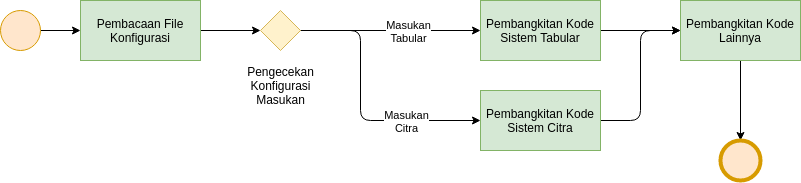
\includegraphics[width=\textwidth]{04-alur-pembacaan-konfigurasi.drawio.png}
    \caption{Alur Pembacaan Konfigurasi oleh Kakas}\label{fig:04-flowchart-config-read}
\end{figure}

Berdasarkan bagian sebelumnya, kakas memodelkan konfigurasi kakas secara internal.
Masing-masing bagian konfigurasi dimodelkan secara terpisah untuk tiap bagian dari konfigurasi.
Konfigurasi juga didefinisikan seumum mungkin agar mudah untuk melakukan penambahan pada fungsionalitas kakas secara mudah.


\subsection{Pembangkitan dan Penggabungan Kode}

\begin{figure}[H]
    \centering
    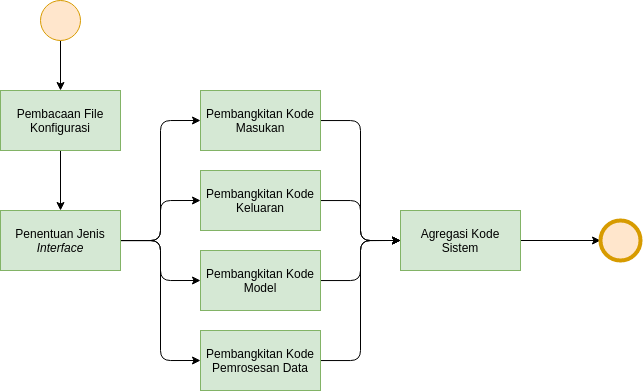
\includegraphics[width=\textwidth]{04-alur-pembangkitan-umum.drawio.png}
    \caption{Alur Pembangkitan oleh Kakas}\label{fig:04-flowchart-code-generation}
\end{figure}

Secara umum, pembangkitan kode dilakukan dalam beberapa tahap seperti yang dideskripsikan pada Gambar~\ref{fig:04-flowchart-code-generation}:
\begin{enumerate}
    \item Penentuan jenis \textit{interface}
    \item Pembangkitan kode masukan
    \item Pembangkitan kode keluaran
    \item Pembangkitan kode model
    \item Pembangkitan kode pemrosesan data
    \item Agregasi kode
\end{enumerate}

Keseluruhan proses pembangkitan kode ini dilakukan melalui penerimaan masukan yang diperlukan untuk masing-masing bagian kode.
Kemudian, dengan masukan serta \textit{template} untuk bagian kode tersebut dapat dibangkitkan sepotong kode.
Sepotong kode akan dikembalikan oleh fungsi dan disimpan untuk digabungkan. 

Bagian sebelumnya telah membahas lebih detail tentang bagaimana bagian-bagian konfigurasi bertanggung jawab terhadap bagian kode dan keterkaitannya dengan masing-masing kode.
Bila disederhanakan, kelima tahapan tersebut dapat mencakup seluruh proses pembangkitan kode.
Akibat dibangkitkan secara terpisah, diperlukan tahapan tambahan untuk menggabungkan kode.

Agregasi kode pada dasarnya menggunakan implementasi yang serupa pada pembangkitan bagian-bagian kode, yaitu menerima masukan nilai-nilai yang diperlukan; dalam hal ini adalah kode yang telah dibangkitkan, serta \textit{template} yang membentuk kode utama sistem.
Segala hal yang berkaitan bagaimana \textit{framework} yang dipilih dibangun berada dalam tahapan ini.
\textit{Endpoint} didefinisikan dalam tahapan ini.
Sebuah \textit{endpoint} dibangun dari potongan-potongan kode yang telah dibangun sebelumnya.

\subsection{Pembangkitan File Terkait}

Selain dari membangkitkan kode, diperlukan beberapa file lagi untuk memastikan sistem ini dapat berjalan.
Beberapa file yang penulis tetapkan untuk dibuat adalah seperti berikut:

\begin{enumerate}
    \item File Dockerfile; dibuat agar sistem bisa dijalankan melalui \textit{container}.
    \item File Gitignore; dibuat untuk memudahkan pengguna bila kode akan dimasukkan ke dalam \textit{version control system}.
    \item File Kakas Python/requirements.txt; dibuat agar diketahui apa saja kakas-kakas yang diperlukan.
\end{enumerate}

Pembangkitan file-file ini dilakukan oleh penulis dengan mekanisme yang sederhana untuk kakas ini.
Dibuat \textit{template} dari file-file yang diperlukan yang akan dibaca oleh kakas dan dibangkitkan setelah semua proses sebelumnya selesai.
Pendekatan ini memiliki kelemahan karena proses ini tidak dilakukan secara modular.
Implementasi kakas menekankan pada pembangkitan kode yang modular saja.